%%
%% Copyright 2007, 2008, 2009 Elsevier Ltd
%%
%% This file is part of the 'Elsarticle Bundle'.
%% ---------------------------------------------
%%
%% It may be distributed under the conditions of the LaTeX Project Public
%% License, either version 1.2 of this license or (at your option) any
%% later version.  The latest version of this license is in
%%    http://www.latex-project.org/lppl.txt
%% and version 1.2 or later is part of all distributions of LaTeX
%% version 1999/12/01 or later.
%%
%% The list of all files belonging to the 'Elsarticle Bundle' is
%% given in the file `manifest.txt'.
%%

%% Template article for Elsevier's document class `elsarticle'
%% with numbered style bibliographic references
%% SP 2008/03/01
%%
%%
%%
%% $Id: elsarticle-template-num.tex 4 2009-10-24 08:22:58Z rishi $
%%
%%
%%\documentclass[preprint,12pt,3p]{elsarticle}
\documentclass[12pt,3p]{elsarticle}
%% Use the option review to obtain double line spacing
%% \documentclass[preprint,review,12pt]{elsarticle}

%% Use the options 1p,twocolumn; 3p; 3p,twocolumn; 5p; or 5p,twocolumn
%% for a journal layout:
%% \documentclass[final,1p,times]{elsarticle}
%% \documentclass[final,1p,times,twocolumn]{elsarticle}
%% \documentclass[final,3p,times]{elsarticle}
%% \documentclass[final,3p,times,twocolumn]{elsarticle}
%% \documentclass[final,5p,times]{elsarticle}
%% \documentclass[final,5p,times,twocolumn]{elsarticle}

%% if you use PostScript figures in your article
%% use the graphics package for simple commands
%% \usepackage{graphics}
%% or use the graphicx package for more complicated commands
%% \usepackage{graphicx}
%% or use the epsfig package if you prefer to use the old commands
%% \usepackage{epsfig}

%% The amssymb package provides various useful mathematical symbols
\usepackage{amssymb}
\usepackage[spanish]{babel}
\usepackage[utf8]{inputenc}
\usepackage{graphicx}
\usepackage{amsmath}
\usepackage{subfigure} 
\usepackage{float}
% For algorithms
\usepackage{algorithm}
\usepackage{algorithmic}


%% The amsthm package provides extended theorem environments
%% \usepackage{amsthm}

%% The lineno packages adds line numbers. Start line numbering with
%% \begin{linenumbers}, end it with \end{linenumbers}. Or switch it on
%% for the whole article with \linenumbers after \end{frontmatter}.
%% \usepackage{lineno}

%% natbib.sty is loaded by default. However, natbib options can be
%% provided with \biboptions{...} command. Following options are
%% valid:

%%   round  -  round parentheses are used (default)
%%   square -  square brackets are used   [option]
%%   curly  -  curly braces are used      {option}
%%   angle  -  angle brackets are used    <option>
%%   semicolon  -  multiple citations separated by semi-colon
%%   colon  - same as semicolon, an earlier confusion
%%   comma  -  separated by comma
%%   numbers-  selects numerical citations
%%   super  -  numerical citations as superscripts
%%   sort   -  sorts multiple citations according to order in ref. list
%%   sort&compress   -  like sort, but also compresses numerical citations
%%   compress - compresses without sorting
%%
%% \biboptions{comma,round}

% \biboptions{}


\journal{--}

\begin{document}

\begin{frontmatter}

\title{Análisis del Generador Renyi Map.}



\author{Marcos Daniel Calderón Calderón}



\ead{marcos.calderon@cimat.mx}




\begin{abstract}
Se explican algunas generalidades del método de Renyi Map. Y se dan algunos resultados de su rendimiento.
\end{abstract}

%\begin{keyword}
%% keywords here, in the form: keyword \sep keyword
%Mapa  \sep \LaTeX \sep Generador no lineal

%\end{keyword}

\end{frontmatter}

\section{Introducción.}
Un paso importante en cualquier sistema de encriptacion caótica es la selección del mapa. Los mapas caóticos tienen diferentes comportamientos en complejidad, propiedades, sensibilidad a las condiciones iniciales, reacción a las perturbaciones aplicadas. Es deseable tener alguna independencia entre el criptosistema y el mapa caótico. 

El generador no Lineal conocido como Renyi Map tiene la siguente forma:

\begin{equation}
\begin{aligned}
f(k)= 2^{n}\tilde{\phi}_{\beta}(2^{-n}k)=\lfloor \beta \cdot k \quad mod \quad 2^{n}  \rfloor \\
=\lfloor  \beta \cdot k  \rfloor \quad 2^{n}.
\end{aligned}
\end{equation}


Otra forma de ver la expresión anterior es de la siguiente manera:

\begin{equation}
f(k)= \left(  q2^{n-i}k + \lfloor \frac{k}{2^{j}} \rfloor \right)  \mod{2^{n}}  
\end{equation}

Los mapas que se generan por medio del Método de Renyi Map, se aplican en Criptografía de la siguiente manera:
\begin{equation}
X_{n}= f(X_{n-1})= \lfloor \lambda \cdot X_{n-1}  \rfloor \mod{2^{PR}} 
\end{equation}

donde $1<\lambda \in \mathbf{R}$  y $X \in {1, 2,...., 2^{PR}-1}$. La expresión anterior puede ser implementado utilizando aritmética de enteros, solo se necesita una multiplicación, una suma y una operación de desplazamiento a la derecha. Un total de $PR \cdot 2^{PR}$ mapas diferentes son definidos en la ecuacion anterior. Con un periodo máximo de $2^{PR}-1$. 

\section{Generadores de números pseudoaleatorios.}
Los generadores de números pseudoaleatorios se utilizan para generar  imitaciones de variables que tienen una distribución uiniforme sobre el intervalo (0,1)
\section{Algunos conceptos importantes del lenguaje C.}

\begin{enumerate}
\item \textbf{unsigned long} Es un tipo de dato utilizado en C, es una variable para almacenar números en 32 bits (4 bytes). Por el contrario que las variables long estándar, las unsigned long no almacenan números negativos, haciendo que su rango sea de 0 a 4,294,967,295 ($2^{32} - 1$).


\item \textbf{Máscaras.} Son secuencias de bits que tienen la finalidad de ocultar o mostrar bits específicos de otra secuencia de bits. Esto se logra al aplicar un operador lógico a la máscara con la secuencia original.

\item \textbf{Hexadecimales en C.} La representación de Hexadecimales en C se realiza al anteponer los caracteres ''0x'' al número que estará en Hexadecimal.

\item \textbf{Operacion módulo en bits.} A la hora de utilizar esta operación en generación de números pseudoaleatorios, se utiliza la operación lógica de $ \& $ con una máscara de bits. 

\end{enumerate}

\section{Demostraciones.}

Dado $\beta_{0}=b_{0}+\gamma_{0}>1$, existe un conjunto contable infinito de valores racionales $\beta>1$, tal que $\forall k \in A_{n}$  $\lfloor \beta_{o}k \rfloor  \mod{2^{n}} =  \beta k \rfloor  \mod{2^{n}} $
en este caso $b_{0}$ es un entero, y $\gamma_{0}$ es una fracción, ademas,  ($A_{n}= k \in \mathbf{N}, 0 \leq k \leq 2^{n}$),
 

\section{Resultados.}
A continuación se muestran algunos resultados acerca del comportamiento del Generador Renyi Map, se muestran los parámetros que se han utilizado y también en qué momento se ha encontrado un ciclo.

\subsection{Ejemplo 1. Elegir el valor del parámetro de manera arbitaria.}
En este ejemplo se eligió el valor del parámetro $\beta$ de una manera arbitraria, esto significa que no se siguieron los criterios definidos por [1] para obtener un buen tamaño de ciclo, también se eligió el valor de $j=15$. Los resultados obtenidos se muestran en la gráfica y en la tabla siguiente.

\begin{figure}[H]
\centering
\subfigure{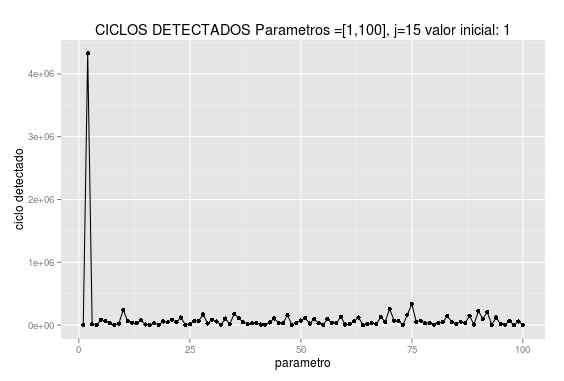
\includegraphics[width=15cm]{gar.jpeg}}
\caption{Gráfica de Ciclos con Parámetros arbitrarios para $\beta$.} \label{Param}
\end{figure}






\subsection{Ejemplo 2. Parámetros dados por [1]: $ n=15$, $ i=j=14$, $ q=[501,701]$,  .}
En este ejemplo, el rango de $q$ es de 501 a 701, pero solo se toman los valores impares. Los resultados obtenidos fueron los siguientes.


\begin{figure}[H]
\centering
\subfigure{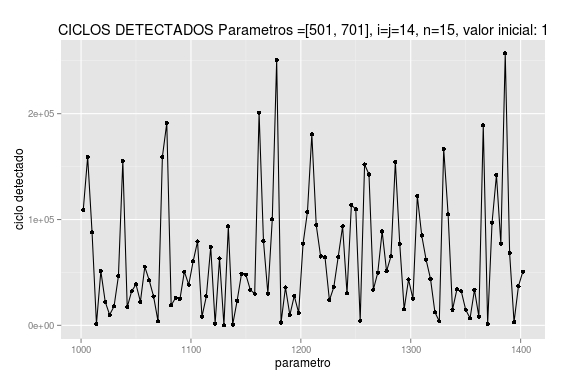
\includegraphics[width=15cm]{ci1.jpeg}}
\caption{Gráfica de Ciclos con las especificaciones:  $ n=15$, $ i=j=14$, $ q=[501,701]$.} \label{Param2}
\end{figure}

Como se puede ver en la gráfica anterior, el tamaño promedio del ciclo depende mucho de las especificaciones dadas, al especificar $n=15$, el tamaño del ciclo disminuye. A continuación, vamos a ver una gráfica de ciclos con $n=32$.

\subsection{Ejemplo 3. Se especificaron los siguientes parámetros: $ n=32$, $ i=j=15$, $ q=[1,1001]$.}
En este ejemplo, el rango de $q$ es de 1 a 1001, pero solo se toman los valores impares. Los resultados obtenidos fueron los siguientes.

\begin{figure}[H]
\centering
\subfigure{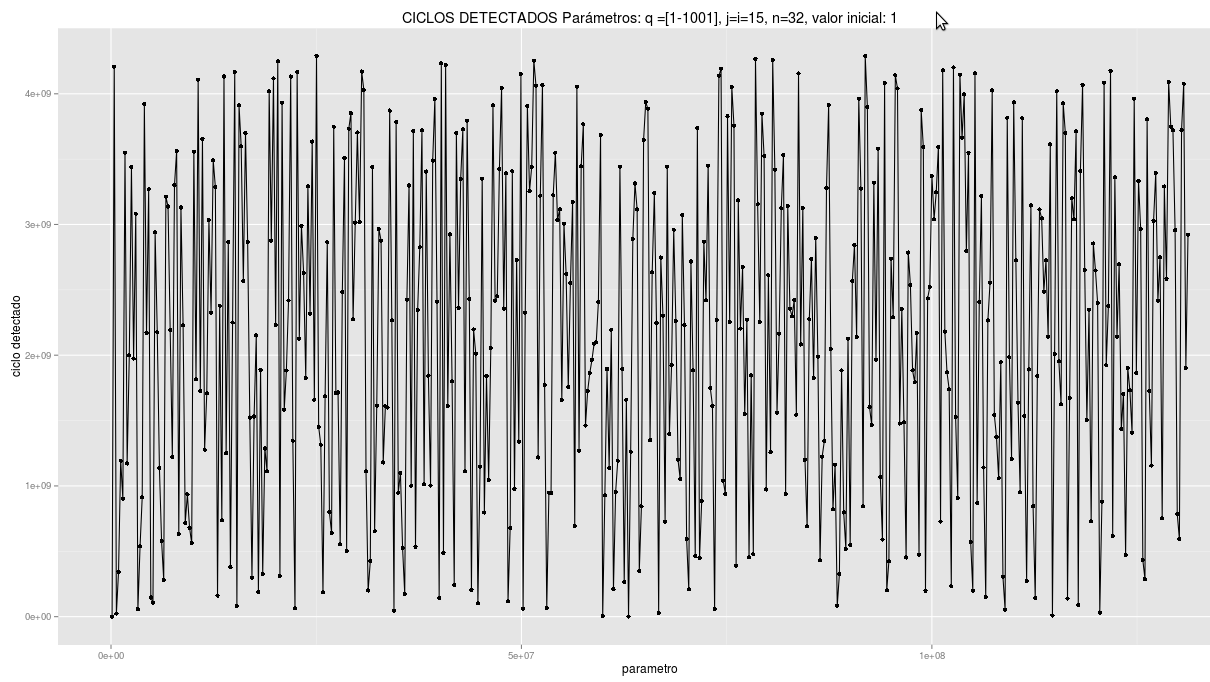
\includegraphics[width=15cm]{ci2.jpg}}
\caption{Gráfica de Ciclos con las especificaciones:  $ n=32$, $ i=j=15$, $ q=[1,1001]$.} \label{Param3}
\end{figure}

Se puede ver que el tamaño de los ciclos ha aumetado de manera considerable, sin embargo, para mayor claridad mostramos una gráfica donde solo se muestran los resultados de $q=[1,101]$, el rango corresponde a 50 parámetros por la restricción de que sólo se toman valores impares para q.

\begin{figure}[H]
\centering
\subfigure{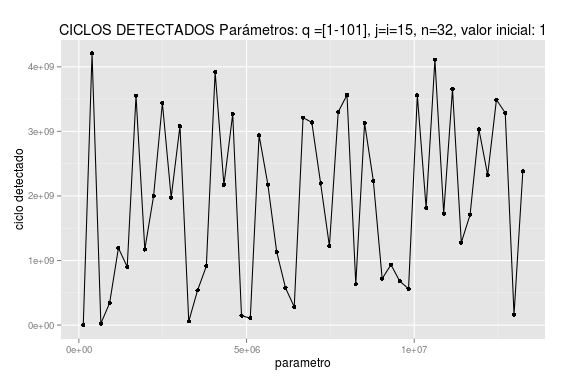
\includegraphics[width=15cm]{reducido.jpeg}}
\caption{Gráfica de Ciclos con las especificaciones:  $ n=32$, $ i=j=15$, $ q=[1,101]$.} \label{Param3}
\end{figure}


\subsection{Ejemplo 4. }
En este ejemplo, el valor de $q$ es de 1 a 101, pero solo se toman los valores impares. También, a comparación del ejemplo anterior, se ha cambiado el valor de i y j. Las especificaciones utilizadas son las siquientes:  $ n=32$, $ i=j=10$, $ q=[1,101]$. La gráfica de resultados muestra que se obtuvieron tamaños de ciclo grandes.



\begin{figure}[H]
\centering
\subfigure{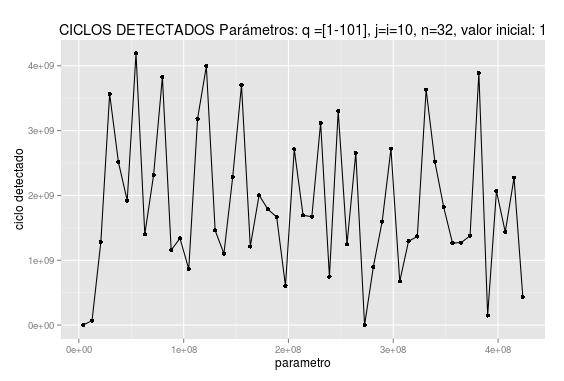
\includegraphics[width=15cm]{r4.jpeg}}
\caption{Gráfica de Ciclos con las especificaciones:  $ n=32$, $ i=j=10$, $ q=[1,101]$.} \label{Param4}
\end{figure}

Como podemos ver, se obtuvieron tamaños de ciclo pequeños, esto se puede deber a muchas causas, pero pensamos que puede ser por la elección de la semilla. Por lo tanto, vamos a elegir una semilla que sea un número primo, en este caso será el número: 2147483647, de hecho este es un número primo de Mersene, porque es igual al valor de una potencia de dos, pero se le resta una unidad. A continuación se muestran los resultados obtenidos, como se puede observar, cuando se utiliza un número primo, se obtienen menos ciclos de corta longitud. A continuación, se muestra una gráfica que nos muestra la diferencia. Sin embargo, no se obtuvo una mejoría notable: en algunos valores poara $q$ el tamaño del ciclo aumenta, pero en otros disminuye.


\begin{figure}[H]
\centering
\subfigure{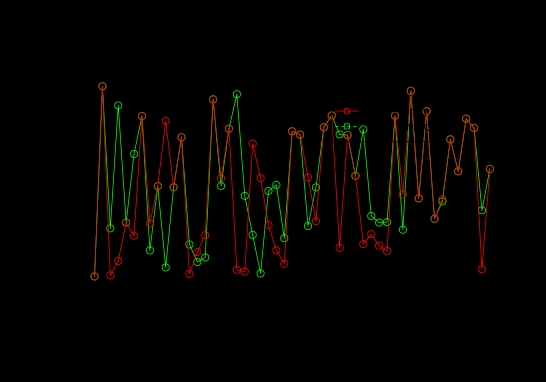
\includegraphics[width=15cm]{uuu.jpeg}}
\caption{Gráfica de Ciclos con las especificaciones:  $ n=32$, $ i=j=10$, $ q=[1,101]$.} \label{Param4}
\end{figure}







\section{Referencias.}

[1] T. Addabbo, M. Alioto, A. Fort, A. Pasini, S. Rocchi and V. Vignoli, A Class of Maximum-Periodo Nonlinear Congruential Generators Derived From the Rényi Chaotic Map. IEEE TRANSACTIONS ON CIRCUITS AND SYSTEMS, 2007.


\end{document}

%%[2] Michael J. Black and Anand Rangarajan, On the Unification of Line Processes, Outlier Rejection, and Robust Statistics with Applications in Early Vision. International Journal of Computer Vision, 1995.
.
%% End of file `elsarticle-template-num.tex'.
